\documentclass[format=sigconf, review=true, screen=true, anonymous=true]{acmart}

\usepackage{siunitx}
\usepackage{graphicx}

\begin{document}

\acmConference[ICMI'17]{International Conference on Multimodal Interaction}{November 2017}{Glascow, Scotland}

\title[SHORT TITLE]{LONG TITLE}
\subtitle{SUBTITLE}

\author{Jacobus C. Lock}
\affiliation{%
  \institution{University of Lincoln}
  \department{School of Computer Science}
  \streetaddress{Brayford Pool}
  \city{Lincoln}
  \state{Lincolnshire}
  \postcode{LN6 7TS}
  \country{United Kingdom}}
\email{jlock@lincoln.ac.uk}

\author{Grzegorz Cielniak}
\affiliation{%
  \institution{University of Lincoln}
  \department{School of Computer Science}
  \streetaddress{Brayford Pool}
  \city{Lincoln}
  \state{Lincolnshire}
  \postcode{LN6 7TS}
  \country{United Kingdom}}
\email{gcielniak@lincoln.ac.uk}

\author{Nicola Bellotto}
\affiliation{%
  \institution{University of Lincoln}
  \department{School of Computer Science}
  \streetaddress{Brayford Pool}
  \city{Lincoln}
  \state{Lincolnshire}
  \postcode{LN6 7TS}
  \country{United Kingdom}}
\email{nbellotto@lincoln.ac.uk}

\thanks{THANKS}

\terms{KEY TERMS}
\keywords{KEY WORDS}

\acmYear{2017}
\received{May 2017}

\maketitle

\begin{abstract}
  hello
\end{abstract}

\section{Introduction}

What is the problem? reference AAAI paper
What is the contribution of this paper?

The UK's Royal National Institute for the Blind (RNIB), a leading organisation in the area, has identified a number of challenges for the modern blind and visually impaired (henceforth referred to as the VI) person. These include the latter's ability to safely and independently use public transport and navigate in unfamiliar environments~\cite{rnib-objectives}. Recent technological advances in the fields of mobile computing and computer vision have allowed for new and innovative solutions to come to the fore to address these challenges. 

To this end, we have proposed a mobile device-based navigation system that caters to the needs of the blind and visually impaired that is based on a Google Project Tango device {CITE AAAI PAPER}. A Tango-enabled device comes pre-equipped with powerful image-processing, localisation and depth-perception capabilities and is built on top of a standard Android platform, giving us access to the entire set of input/output options that Android has to offer. The proposed system will use multiple feedback modes to guide a user toward a target destination while providing information on any oncoming obstacles.

In this paper, we discuss in detail how one of these feedback modes are used in our system. We also discuss the experiment we performed to determine how effective this mode is at directing a user to completing a given task, as well as how the mode's parameter values affect a user's performance at completing the aforementioned task. 

The remainder of this paper is organised as follows: HOW IS PAPER ORGANISED?

\section{Previous Work}

-interface for the blind (how effective are they, etc)
-spatial sound

\subsection{Navigation}

Delivering a system that will allow the blind and visually impaired (VI) to independently navigate and accomplish everyday tasks is not a new proposal; in fact, there are multiple commercial systems available (besides the traditional walking cane) and academic research for this field dates as far back as [CITE WHEN]. The products vary from sonar, radar and GPS-based systems, to some of the more recent systems which use computer vision techniques to detect and avoid obstacles in the user's path. 

One approach that has been investigated is to outfit the existing white walking cane with various sensors, such as sonar, radar, motor encoders, etc.,~\cite{ulrich1997, marion2008batcane} to detect warn the user of upcoming obstacles from a distance instead of relying on haptic feedback from the impact between the cane and the obstacle. These systems are fairly simple and reliable and are familiar to the VI, but they are typically clunky, advertising the users' disability, which can be a major hurdle to market penetration. Another, more discreet approach, was to equip a normal to act as an radio-frequency identification (RFID) antennae to read a set of RFID tags that are placed around the environment at key spots or along a path~\cite{faria2010electronic, willis2005}. This approach to modifying the traditional cane is more discreet than the systems mentioned earlier and has been shown to work well. However, the major drawback here is the significant cost of modifying existing infrastructure with RFID tags and maintaining them to keep up with a changing environment. GPS systems, such as the Drishti system~\cite{ran2004drishti}, while cheap and reliable in open outdoor environments, are not applicable here since we wish our system to be usable in built-up urban areas and indoors where GPS signals are notoriously unreliable. 

Computer vision-based systems provide a good compromise between usability, cost and accuracy and has has been the focus of much research in the recent past. One popular solution is to use an RGB-D depth sensing camera, which are becoming increasingly more accurate and cheaper, to build a 3D image map which will allow a user to safely traverse through~\cite{lee2015, rodriguez2012obstacle}. However, these systems have not yet been thoroughly tested with VI people in a real environment. Another approach is to use object recognition techniques to detect various objects and landmarks, such as doors, staircases, etc.~\cite{tian2013b}, and communicate their relative location to the user. Furthermore, though not stritcly useful for navigation bu nice to have, are other assistive functionalities, such as facce recognition and currency reading, that can also be added to enhance the VI user's experience and add more usability to the system~\cite{chessa2016}.

\subsection{Interfacing}



\section{Portable Navigation System}

The system we intend to ultimately deliver is a portable navigation device that caters to the needs of the blind by using a combination of different feedback modes to facilitate two-way communication between the user and the device. We use multiple modes to overcome the bandwidth limitation that is introduced when visual data is translated into audio cues and voice commands, for example. 

The system is based on a Google Tango device, which come equipped with an RGB-D camera to estimate depth and combines an inertial measurement unit (IMU) with powerful and robust landmark recognition and image processing algorithms to localise itself and `close the loop'. : a Android-based cellular device which comes pre-equipped with powerful localisation, depth perception and image processing capabilities. Add added benefit of this platform is its familiar, compact form-factor which will help overcome the hurdle of user-acceptance and usability. 

We intent to use multiple feedback modes to provide the VI user with navigation and obstacle avoidance instructions. These modes are spatialised audio, voice prompts and voice cues. However, for this series of experiments, we only employed the spatialised audio mode in order to determine its efficacy. 

\section{Audio Interface}

For the series of experiments we performed, we only used the audio feedback mode to interface with the user. This audio component is responsible for conveying the 3D position of a target relative to the target in terms of pan and tilt angles, as well as distance to the target, using a scheme similar to a polar coordinate system. To simplify the experiment process and better isolate the different variables, we only enabled the pan and tilt parts of the interface, leaving the distance out to be experimented with in the future.  

The audio being generated is a sinusoidal sound wave that is constantly generated and played to the user through bone-conducting headphones. We select a sinusoidal wave due to it being relatively simple to manipulate and analyse. Furthermore, we opted to use an external, bone-conducting headset to play the audio to better simulate the use-case we are designing the system toward where our system will act as a supplementary navigation aid which does not interfere with their other senses; in particular their sense of hearing, which they tend to rely upon heavily [CITE][REVIEW THIS SENTENCE].

\subsection{Pan Description}

The pan angle describes the angle which the user needs to rotate the camera vector around the Y-axis, i.e. how far the target is to the left or right of the user. To communicate this to the user, we use a head-related transfer function (HRTF) to add a spatial element to the audio tone that the system plays to the user, making the tone sound to the user like it's coming from the direction of the target. 

The HRTF functionality is implemented using the OpenAL library [CITE] to generate a sinusoidal sound wave based on the relative difference in the user and target's positions. We implement the library as a `black box' where the inputs are positions and it outputs a tone based on the difference in those positions, implying that we don't have access to the internal parameters of the HRTF. We therefore implemented the same HRTF across all of the experiments we conducted.  

OpenAL is able to generate a 3D spatial tone (pan, tilt and distance). However, we opted to only use it to convey the pan dimension and use other tools to convey the distance and tilt dimensions. We selected this approach partly because HRTFs commonly have difficulty communicating the tilt angle effectively [CITE]. Furthermore, implementing other options for the distance and tilt dimensions grants us finer control over how they are communicated to the user.

\subsection{Tilt Description}

To enable the system to communicate the tilt direction of the target, the system adjusts the emitted tone's pitch as a logarithmic function of the elevation angle, $\theta$, between the user's camera vector and the target's position. Here, a high pitch means the target is above the camera vector and the user should look up, whereas a low pitch means the target is below the camera vector and the user should look down. This high/low association scheme is selected, because humans naturally tend to associate high-pitched sounds with higher objects and lower-pitched noises with lower objects [CITE]. We also opt for a logarithmic, octave-based gain function for the pitch because it sounds more natural to the human ear [CITE].

We wish to determine what effect the gradient of the pitch gain function has on a user's performance; that is to say, does an increased rate of change in the pitch as a function of the elevation angle lead to an increased target acquisition rate, for example. For this we select three different pitch gain gradients, so-called low, median and high gain presets. To find these gradients, we set the maximum and minimum limits for the pitch and the elevation angles. Furthermore, for the sake of consistency, each gradient is set to pass through the same pitch value at the \SI{0}{\radian} elevation angle.   

The neutral, \SI{0}{\radian}, position is set to be directly in front of the user and we limit the angles between $\pm$\SI[quotient-mode=fraction]{\pi / 2}{\radian}, requiring the system to be able to communicate angles within a range of \SI{\pi}{\degree}. Anything outside of this range implies that the target is behind the user. 

After practical tests with the Tango and the headphones, we set the neutral, on-target tone to a frequency of \SI{512}{\hertz} for its audibility. For the median preset, we set the maximum and minimum pitches to be two octaves higher and lower than the neutral tone, giving limits of \SI{2048}{\hertz} and \SI{128}{\hertz} respectively. The low preset is set to one octave higher and lower than the neutral tone (\SI{1024}{\hertz} and \SI{256}{\hertz}) and the hight to 3 octaves higher and lower (\SI{4096}{\hertz} and \SI{64}{\hertz} than the neutral tone. We selected these limits partially more practical reasons, given the fact that the bone conducting headphones we used have low volume gain at very high and low frequencies, making it difficult to hear. Figure~\ref{fig:pitch-preset-plot} shows the low, median and high gain preset graphs.  

\begin{figure}
  \centering
  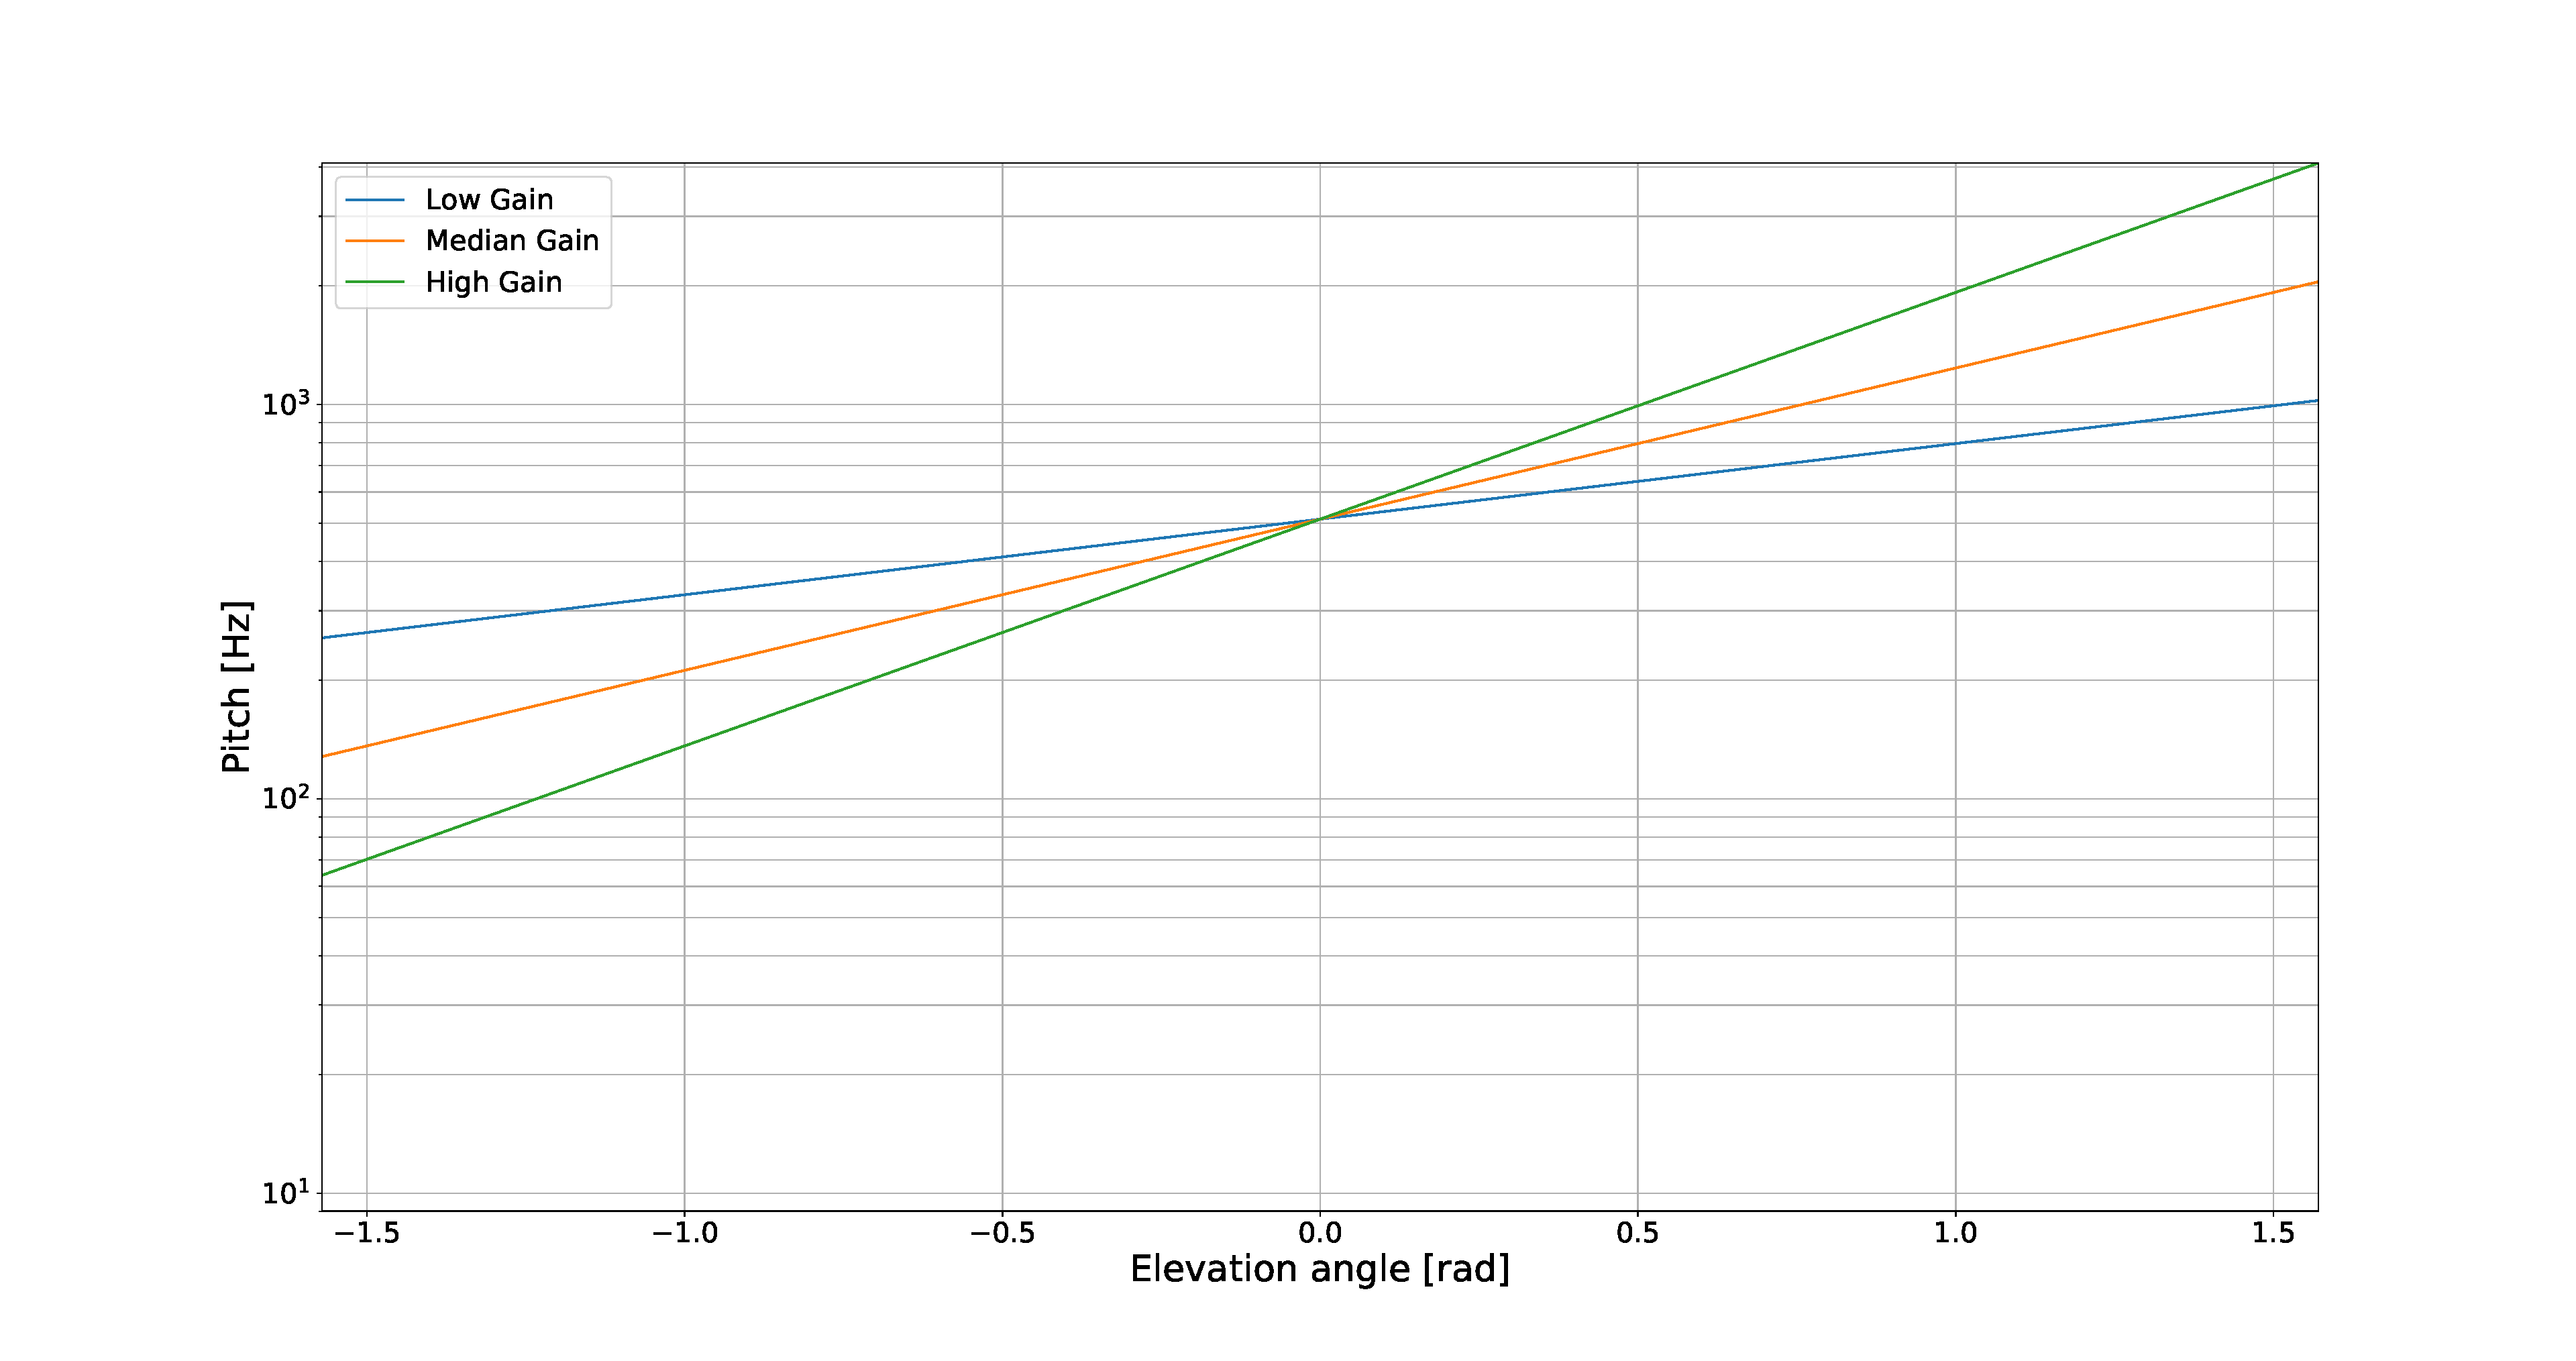
\includegraphics[width=0.5\textwidth]{figures/pitch_gradient.pdf}
  \caption{Plot depicting the different pitch gain preset functions.}
  \label{fig:pitch-preset-plot}
\end{figure}

\section{Tests Performed}

To determine how effective the individual feedback modes of our HMI is at directing a user to perform a given task, we performed a set of experiments with blindfolded users using only a limited set of the feedback modes. The reason for only experimenting with one or two modes together is to simplify the experiment procedure and incrementally build up our knowledge of the interactions between the user and the feedback mode so that we can eventually integrate all of the feedback modes into a single implementation and perform an optimal set of experiments that will provide us with all of the important data that we require. 

In this case, we experimented with the spatialised sound feedback mode; that is to say we determined how effective a spatial tone, with varying pitch, is at directing a user to pan and tilt a camera to find a target. Furthermore, we also carried out a set of pre-screening experiments to determine each subject's hearing characteristics. The following sections will discuss all of these experiments and their objectives in detail. 

\subsection{Test Objectives}

Every subject was asked to participate in 4 different experiments: the first three were pre-screening experiments to evaluate the subjects' hearing characteristics and the last to determine how effective our HMI's spatial sound is at controlling a subject's pan and tilt. Furthermore, we wish to determine how the different values of this spatial sound affects a subject's performance. 

The hearing characteristics we wished to determine were the subjects' spatial awareness, tone limits and tone discrimination capability. For the spatial sound experiment we wish to determine how quickly each subject can find their target's, what each subject's target search strategy is as well as how the different feedback parameter values affect these performances. 

\subsection{Test Procedure}

For the experiments we used 40 blindfolded volunteers and had them perform a series of experiments using our system and a pair of bone conducting headphones. The subjects were recruited on a volunteer-basis and consisted of a diverse group of undergraduate students with ages ranging between [WHAT ARE THE AGES?], with [WHAT ARE THE GENDER NUMBERS?]. The subjects also reported having no significant sight or hearing issues or any other major disability. 

The 40 subjects were asked to participate in 4 experiments, each of which is discussed here.

\subsubsection{Spatial Awareness Test}

In this experiment, we determine a subject's ability to tell the direction a sound is coming from. To do this, we play a 512Hz sinusoidal tone to the candidate through the headphones that comes from either the left or right of the subject. The subject must then select whether the sound source is to the left or right. The sound source location is simulated using a head-related transfer function (HRTF). The longer this experiment is run, the source moves closer to the centre of the subject making it more difficult to localise the sound source. 

For this progressive increase in difficulty, a 2-up, 1-down step process is used, meaning that for every 2 correct answers, the distance to the centre halves, making the process harder. Conversely, it becomes easier for each incorrect answer by doubling the sound source's distance from the centre. We also select to use 2 different step sequences, one starting at a large distance from the user and the other at a close distance, giving us an `easy' and `hard' step respectively. The terminating condition for the experiment is when the 2 step sequences are within 2 step ranges of each other for 3 consecutive guesses. This will give us a distance band within which the candidate is capable of localising the sound source. Each candidate will performed this experiment three times. 

\subsubsection{Pitch Discrimination Test}

For this experiment , we determine a subject's ability to tell tones apart, i.e. how well can they tell if a tone is high or low pitched? Here we play 2 tones to the subjects, one after the other, with one tone being higher or lower-pitched than the other. The subject's were asked to select whether the second tone was higher or lower-pitched than the first tone.

As with the spatial experiment , a 2-up, 1-down step process is used: for every 2 consecutive correct answers, the pitch difference between the two tones will be halved, increasing the difficulty, and the difference is doubled for every incorrect answer, making the tones easier to differentiate. Two step sequences are again used here, one starting with a large pitch difference between the tones and the other with a small difference. The termination condition is when the two step sequences are within one octave of each other for 3 consecutive answers. Each subject performed this experiment twice. 

\subsubsection{Tone Limit Test}

We determined the candidates' tone limits as a final experiment before they took part in the  main, target-finding experiment. We did this by playing a single tone that increases in pitch as time progresses. The candidate was then asked to click a button as soon as he/she started hearing a tone and to click the button again when the tone became inaudible. The subject was then asked to repeat the process 6 times, but the tone direction was reversed after each run, meaning that the tone either started high and went low or started low and went high. 

\subsubsection{Target Search Test}

The final experiment is the main one and will answer the question we are most interested in: how well does a spatial tone direct a user to look in a specific direction, and how do the parameters of this tone affect the user's performance in this task? 

Here a candidate was blindfolded and given a Tango device running an app written specifically for this experiment. When started, a set of virtual targets were presented one at a time to the subject on the Tango's screen. Then, depending on the direction the candidate is currently pointing the camera relative to the target's position, the Tango generates and plays a tone via a bone-conducting headphone to indicate the pan and tilt adjustment the candidate needs to make the camera to face the target. These instructions are a spatialised tone with varying pitch: an HRTF will indicate whether the target is to the left or the right and the pitch will indicate whether the candidate should be looking up (high pitch) or down (low pitch) to find the target. 

Once the candidate pointed the camera toward the target, the HRTF centred the tone in front of the candidate with a neutral pitch of 512Hz, which we used as the `on-target' pitch for all of our experiment (the candidates were given a few minutes without a blindfold where they could familiarise themselves with the system where they could confirm the target's location with their own eyes). However, the candidate had to decide for themselves whether they truly were looking at the target and tap the screen to indicate the location they believe to be in (i.e. the current location they are looking at). At this point a new target is presented to the candidate which they had to search for again. 28 targets are presented to each subject per round. 

After every round of these experiments, the parameters controlling the tone's behaviour were adjusted. In this case, the rate of change of the tone's pitch was adjusted to make the pitch increase at a lower or higher rate as a function of the elevation angle between the target and the candidate's current looking direction. This was done to see whether, for example, a more rapid increase in pitch will help the candidate find the target faster. 

For this experiment, the distance between the candidate and the target is not considered here. Therefore, the target's are generated on a plane at a constant distance from the candidate, in this case 2m. Throughout the experiment, various parameters of the target and the candidate are recorded and streamed in real-time to a laptop computer via a WiFi connection.

\section{Results}

\section{Discussion}

\section{Future Work}

\section{Conclusion}

\bibliographystyle{ACM-Reference-Format}
\bibliography{icmi17}

\end{document}
